\chapter{Architetture dei Modelli}
\label{chap:architetture}

Questo capitolo descrive le architetture dei modelli utilizzati nel progetto: il teacher 3D ResNet-50, lo student MobileNet3D e il meccanismo di accoppiamento dei layer per l'Attention Transfer.

\begin{figure}[H]
    \centering
    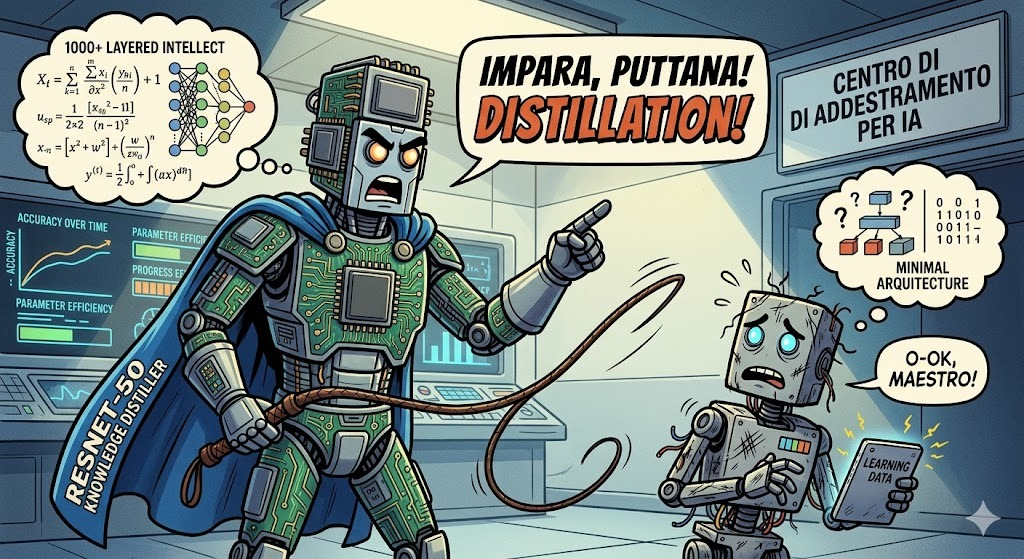
\includegraphics[width=0.7\textwidth]{parts/cap3_architetture/distil.jpeg}
    \caption{Schema concettuale della Knowledge Distillation: il modello teacher pesante trasferisce la propria conoscenza allo student leggero attraverso soft targets e, opzionalmente, mappe di attenzione intermedie.}
    \label{fig:kd_schema}
\end{figure}

\section{Teacher: 3D ResNet-50 (\texttt{slow\_r50})}

Il modello teacher è la variante \texttt{slow\_r50} di PyTorchVideo~\cite{feichtenhofer2019slowfast}, un 3D ResNet-50~\cite{he2016deep} pre-addestrato su Kinetics-400~\cite{kay2017kinetics}. L'architettura è composta da 6 blocchi sequenziali (indici 0--5):

\begin{table}[H]
\centering
\caption{Struttura del Teacher (slow\_r50). Il blocco 5 è la testa di classificazione, non uno stage di estrazione feature.}
\label{tab:teacher_blocks}
\begin{tabular}{cccc}
\toprule
\textbf{Blocco} & \textbf{Tipo} & \textbf{Output Shape} & \textbf{Descrizione} \\
\midrule
0 & ResStage & $[B, 64, T, 56, 56]$ & Conv iniziale + pool \\
1 & ResStage & $[B, 64, T, 56, 56]$ & Primo stage residuale \\
2 & ResStage & $[B, 256, T, 28, 28]$ & Secondo stage residuale \\
3 & ResStage & $[B, 512, T, 14, 14]$ & Terzo stage residuale \\
4 & ResStage & $[B, 1024, T, 7, 7]$ & Quarto stage residuale \\
5 & ResNetBasicHead & $[B, 101]$ & Global avg pool $\rightarrow$ proj \\
\bottomrule
\end{tabular}
\end{table}

La testa di classificazione originale (pre-addestrata su 400 classi Kinetics) viene sostituita con un layer lineare a 101 uscite per UCF-101. Il pooling spaziale-temporale viene reso adattivo (\texttt{AdaptiveAvgPool3d(1,1,1)}) per supportare qualsiasi dimensione di input. Il fine-tuning utilizza SGD con learning rate 0.0007, weight decay $10^{-3}$, batch size 12 e scheduler cosine annealing per 50 epoche.

\section{Student: MobileNet3D}

Lo student è un'architettura MobileNetV2~\cite{sandler2018mobilenetv2} adattata alle convoluzioni 3D per l'elaborazione video. L'architettura si basa su blocchi \textit{Inverted Residual} 3D con convoluzioni depthwise separabili:

\begin{enumerate}
    \item \textbf{Pointwise Expansion}: convoluzione $1\times1\times1$ che espande i canali di un fattore $t$ (expansion ratio).
    \item \textbf{Depthwise 3D Convolution}: convoluzione $3\times3\times3$ con \texttt{groups=hidden\_dim}, che processa ciascun canale indipendentemente. Lo stride temporale è sempre 1, preservando la dimensione $T$.
    \item \textbf{Pointwise Projection}: convoluzione $1\times1\times1$ che proietta al numero di canali di output, senza attivazione (\textit{linear bottleneck}).
\end{enumerate}

\begin{table}[H]
\centering
\caption{Stage del MobileNet3D con le risoluzioni spaziali di output.}
\label{tab:student_stages}
\begin{tabular}{cccccc}
\toprule
\textbf{Stage} & \textbf{$t$} & \textbf{$c$} & \textbf{$n$} & \textbf{$s$} & \textbf{Output Shape} \\
\midrule
0 & 1  & 16  & 1 & 1 & $[B, 16, T, 56, 56]$ \\
1 & 6  & 24  & 2 & 2 & $[B, 24, T, 28, 28]$ \\
\textbf{2} & \textbf{6}  & \textbf{32}  & \textbf{3} & \textbf{2} & $[B, 32, T, 14, 14]$ \\
3 & 6  & 64  & 4 & 2 & $[B, 64, T, 7, 7]$ \\
\textbf{4} & \textbf{6}  & \textbf{96}  & \textbf{3} & \textbf{1} & $[B, 96, T, 7, 7]$ \\
5 & 6  & 160 & 3 & 2 & $[B, 160, T, 4, 4]$ \\
\textbf{6} & \textbf{6}  & \textbf{320} & \textbf{1} & \textbf{1} & $[B, 320, T, 4, 4]$ \\
\bottomrule
\end{tabular}
\end{table}

dove $t$ è l'expansion ratio, $c$ i canali di output, $n$ il numero di blocchi e $s$ lo stride spaziale. Gli stage evidenziati in grassetto sono quelli utilizzati per l'Attention Transfer.

Il classificatore è composto da una convoluzione finale $1\times1\times1$ a 1280 canali, adaptive average pooling 3D, dropout (0.2) e un layer lineare a 101 classi. Il training del baseline utilizza AdamW~\cite{loshchilov2019adamw} con learning rate 0.0005, weight decay 0.01 e cosine annealing per 60 epoche.

\section{Confronto Dimensionale}

\begin{table}[H]
\centering
\caption{Confronto tra Teacher e Student in termini di parametri, dimensione e latenza di inferenza.}
\label{tab:model_comparison}
\begin{tabular}{lccc}
\toprule
\textbf{Modello} & \textbf{Parametri} & \textbf{Dimensione (MB)} & \textbf{Latenza (ms)} \\
\midrule
3D ResNet-50 (Teacher) & $\sim$33.4M & $\sim$128 & -- \\
MobileNet3D (Student)  & $\sim$2.5M  & $\sim$9.5 & $\sim$1.8 \\
\bottomrule
\end{tabular}
\end{table}

Il rapporto di compressione è superiore a \textbf{13$\times$} in termini di parametri e \textbf{13$\times$} in dimensione del modello, rispettando ampiamente il target di 5--10$\times$ richiesto dal track.

\section{Accoppiamento dei Layer per l'Attention Transfer}
\label{sec:layer_pairing}

L'accoppiamento corretto tra i layer del teacher e quelli dello student è cruciale per un efficace Attention Transfer. La scelta è guidata dalla similitudine semantica e dalla compatibilità delle risoluzioni spaziali:

\begin{table}[H]
\centering
\caption{Accoppiamento delle feature map per l'Attention Transfer.}
\label{tab:feature_pairing}
\begin{tabular}{ccccc}
\toprule
\textbf{Coppia} & \textbf{Teacher} & \textbf{Shape Teacher} & \textbf{Student} & \textbf{Shape Student} \\
\midrule
1 & Blocco 2 & $[B, 256, T, 28, 28]$ & Stage 2 & $[B, 32, T, 14, 14]$ \\
2 & Blocco 3 & $[B, 512, T, 14, 14]$ & Stage 4 & $[B, 96, T, 7, 7]$  \\
3 & Blocco 4 & $[B, 1024, T, 7, 7]$ & Stage 6 & $[B, 320, T, 4, 4]$ \\
\bottomrule
\end{tabular}
\end{table}

Si noti che la dimensione temporale $T$ è identica tra teacher e student a tutti i livelli, poiché entrambi i modelli utilizzano stride temporale pari a 1. Questo permette un trasferimento diretto dell'attenzione temporale senza interpolazione. Le differenze nelle risoluzioni spaziali (es. $28\times28$ vs $14\times14$) vengono gestite tramite interpolazione bilineare 2D, come descritto nella Sezione~\ref{sec:at_bug}.
